\documentclass{uebblatt}

\DeclareMathOperator{\sd}{sd}

\begin{document}

\maketitle{11}{}

\begin{aufgabe}{Ein erster Einblick in Homotopiepushouts}
\begin{enumerate}
\item Zeige anhand eines Beispiels in~$\Top$, dass folgende wünschenswerte
Aussage im Allgemeinen falsch ist: Sei~$X \leftarrow A \rightarrow Y$ ein
Diagramm. Sei~$X' \leftarrow A' \rightarrow Y'$ ein dazu schwach äquivalentes
Diagramm. Dann ist auch der Pushout~$X \amalg_A Y$ schwach äquivalent zu~$X'
\amalg_{A'} Y'$.
\end{enumerate}
Der \emph{Homotopiepushout} eines Diagramms~$X \leftarrow A \rightarrow
Y$ in einer Modellkategorie ist per Definition der Pushout eines schwach
äquivalenten Diagramms~$X' \leftarrow A' \rightarrow Y'$, in dem~$A'$ kofasernd
und die beiden Morphismen Kofaserungen sind.
\begin{enumerate}
\addtocounter{enumi}{1}
\item Zeige, dass der Homotopiepushout bis auf schwache Äquivalenz
wohldefiniert ist.
\item Sei die Modellkategorie linkseigentlich und sei einer der Morphismen~$X
\leftarrow A$ und~$A \rightarrow Y$ eine Kofaserung. Zeige, dass dann der
Homotopiepushout und der gewöhnliche Pushout übereinstimmen.
% http://ncatlab.org/nlab/show/proper+model+category
% http://www-home.math.uwo.ca/~jardine/papers/HomTh/lecture007.pdf, S. 7
\end{enumerate}
\end{aufgabe}

\begin{aufgabe}{Fasernder Ersatz durch baryzentrische Unterteilung und Erweiterung}
Die \emph{baryzentrische Unterteilung}~$\sd \Delta[n]$ von~$\Delta[n]$ ist der
Nerv der Partialordnung der nichtdegenerierten Simplizes von~$\Delta[n]$. Wir
definieren einen Funktor~$\mathrm{Ex} : \sSet \to \sSet$
durch~$\mathrm{Ex}(X)_n \defeq \Hom_\sSet(\sd \Delta[n], X)$.
\begin{enumerate}
\item Wie sehen~$\sd \Delta[1]$ und~$\sd \Delta[2]$ aus?
\item Gib den kanonischen Morphismus~$j_X : X \to \mathrm{Ex}(X)$ an.
\item Zeige, dass sich alle Hörner von~$\mathrm{Ex}(X)$ in~$\mathrm{Ex}^2(X)$
füllen lassen.
\item Folgere, dass der Kolimes von~$X \to \mathrm{Ex}(X) \to
\mathrm{Ex}^2(X) \to \cdots$ ein Kan-Komplex ist.
\end{enumerate}
\end{aufgabe}
% http://www.ms.uky.edu/~guillou/KanEx.pdf

\begin{aufgabe}{Anodynizität von Kofaserungen}
Zeige: Eine Kofaserung zwischen simplizialen Mengen (bezüglich der
Quil\-len-Mo\-dell\-struk\-tur) ist genau dann anodyn, wenn sie eine schwache
Äquivalenz ist.
\end{aufgabe}

\begin{aufgabe}{Fundamentalgruppe der eindimensionalen Sphäre}
Berechne~$\pi_1(\SS^1)$.
\end{aufgabe}

\begin{aufgabe}{Erzeugnis unter beliebigen vs. filtrierten Kolimiten}
Sei~$S$ eine Menge~$\kappa$-kompakter Objekte in einer kovollständigen
Kategorie~$\C$. Sei jedes Objekt aus~$\C$ kleiner Kolimes von Objekten aus~$S$.
Zeige, dass jedes Objekt aus~$\C$ dann ein~\emph{$\kappa$-fil\-trierter} Kolimes
von Objekten aus~$\overline{S}$ ist, wobei~$\overline{S}$ der Abschluss von~$S$
unter~$\kappa$-kleinen Kolimiten ist.
\end{aufgabe}
% http://math.stackexchange.com/questions/717113/definition-of-locally-presentable-category

\centering
\href{http://www.4teachers.de/?action=keywordsearch&searchtype=images&searchstring=Kinder%C3%BCberraschung}{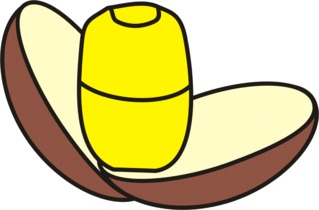
\includegraphics[scale=0.25]{images/ueberraschungsei}}
\par

\end{document}
